
\documentclass[12pt]{amsart}
\usepackage{amsthm,amssymb,amsfonts,epic,epsfig,framed,fullpage,latexsym,enumerate}
%\usepackage{framed}

\usepackage{xcolor}
\usepackage{comment}
\usepackage{multirow}
\usepackage{float}
\usepackage{graphicx}
\usepackage{tikz-qtree}
\usepackage{algorithmic}

\newcommand\TT[1]{\texttt{#1}}

\newcommand{\adj}{\ensuremath{\mathrm{adj}}}

\newcommand{\Length}{\ensuremath{\mathtt{length}}}
\newcommand{\Jmin}{\ensuremath{\mathtt{jmin}}}
\newcommand{\Min}{\ensuremath{\mathtt{min}}}
\newcommand{\total}{\ensuremath{\mathtt{total}}}
\newcommand{\DEG}{\ensuremath{\mathtt{deg}}}
\newcommand{\NGN}{\ensuremath{\mathtt{numGreyNbrs}}}
\newcommand{\COLOR}{\ensuremath{\mathtt{color}}}
\newcommand{\white}{\ensuremath{\mathtt{white}}}
\newcommand{\grey}{\ensuremath{\mathtt{grey}}}

\newcommand{\pred}{\ensuremath{\mathtt{pred}}}
\newcommand{\usp}{\ensuremath{\mathtt{usp}}}
\newcommand{\true}{\ensuremath{\mathtt{true}}}
\newcommand{\false}{\ensuremath{\mathtt{false}}}

\newcommand{\opt}{\ensuremath{\mathtt{opt}}}

\newcommand{\dist}{\ensuremath{\mathtt{dist}}}
\newcommand{\length}{\ensuremath{\mathtt{length}}}
\newcommand{\Right}{\ensuremath{\mathtt{right}}}
\newcommand{\Left}{\ensuremath{\mathtt{left}}}
\newcommand{\Middle}{\ensuremath{\mathtt{middle}}}

% Comments & responses (main text)
\newcommand{\comm}[1]{\marginpar{\textsl{\color{red} #1}}}
\newcommand{\commB}[1]{\marginpar{\textsl{\color{blue} #1}}}

\newtheorem{lemma}{Lemma}
%\usepackage{fullpage}
\usepackage{newtxtext,newtxmath}
%\usepackage{times,inconsolata}

\usepackage[titlenotnumbered,linesnumbered,noline,ruled,noend]{algorithm2e}

\DeclareMathOperator{\val}{value}
\DeclareMathOperator{\capac}{cap}

\SetKwProg{Fn}{}{}{}
\SetKwFunction{greedyMIS}{greedyMIS}%

\mathchardef\mhyphen="2D

\newcounter{pNum}


\newcommand{\problem}[2]{\addtocounter{pNum}{1}
\section*{Problem \arabic{pNum}: #1 (#2 Points)}}

\begin{document}

\tikzset{every tree node/.style={minimum width=2em,draw,circle},
         blank/.style={draw=none},
         edge from parent/.style=
         {draw,edge from parent path={(\tikzparentnode) -- (\tikzchildnode)}},
         level distance=1.5cm}
%\thispagestyle{empty}

%\hspace{0.11cm} \vspace{2cm}

\title{
Computer Science 311\\
Spring 2020\\
Final Exam \\
}

\maketitle


%\vspace{1cm}

\section*{Instructions}

\begin{itemize}
\item
You have {\bf 30} hours to complete the exam, including the uploading time of your solutions. 
\item 
There are four questions and one bonus question. The maximum possible score is 70; the number of points for each problem is indicated on the next page.
\item
Read all questions carefully before starting.
\item
Since the exam is conducted remotely, questions should be asked on {\bf Piazza only}. Note that we do {\bf NOT} answer questions through emails. 
\item All questions should be for clarification purposes only. Please keep your questions concise. We CANNOT have lengthy discussions like we usually answer homework questions on Piazza.
\item Due to the challenges of conducting the exam remotely, we can only try to answer the questions in time when we see them. However, we cannot guarantee how quickly we can respond. If you have questions, please ask early.
\item
We expect clear and concise answers.  Think carefully before you write; make sure that every word you write counts. 
\item
If you do not know the answer to a problem, write ``\emph{I don't know}'' and (except where otherwise stated) you will earn approximately 20\% of the points for that problem.
\item
When asked to provide an algorithm, remember to
\begin{itemize}
\item
describe the algorithm clearly,
\item
analyze the running time of the algorithm.
\end{itemize}
\item For any algorithm, your grade will depend on the efficiency of your algorithm.
\end{itemize}


\vfill


\begin{framed}
\vspace{-0.3cm}
\section*{Write Your Name and Your Recitation Section Number Here}
\begin{center}{\hspace{2cm}} \end{center}
\vspace{1cm}
\end{framed}
\vfill

\newpage

\vfill

\hspace{0cm}

\vfill

\section*{Your Score}

\vfill

\begin{center}
\begin{tabular}{|c|c|c|}
\hline
Problem &
Points &
Score \\ \hline
1 & 15 & \\ \hline
2 & 15 & \\ \hline
3 & 15 & \\ \hline
4 & 15 & \\ \hline
5 (Extra) & 10 & \\ \hline
Total & 60 + 10 = 70 & \\
\hline
\end{tabular}
\end{center}

\vfill

\hspace{0cm}

\vfill

\newpage

\newpage


\problem{Short Questions (NO credit for writing ``I don't know'')}{15}

\begin{enumerate}[(a)]


\item (3 points) {\bf True or False:} Every directed graph can have more than one minimum spanning tree. If true, give a short explanation.
If false, give a counterexample.

\TT{True} 

Its possible to have multiple paths with the same weight. Suppose we have to spanning paths with the same weight then if one of theses paths is a minimum spanning path they both must be minimum spanning. This gives more then one minimum spanning path.

\vfill

\item (3 points) Suppose $G$ is a directed graph with $n$ vertices and $m$ edges, and let $s$ be any vertex in $G$.   

{\bf True or False:} \emph{If every vertex of $G$ is reachable by a directed path from $s$, then $m \ge n-1$ edges.}
If true, give a short explanation.
If false, give a counterexample.

\TT{True} 

\begin{proof}
For a directed graph G lets supports all edges have a weight of 1. Then for there to be a minimal spanning tree. There needs to exist a path from a vertex s $\in G$ to all other nodes. Suppose there isnt a incoming reference to s then there is a n-1 nodes to be connected to s thus there are n-1 outgoing edges in G to have all vertices connected from s. giving us the minimum about of edges needed to have a spanning tree. 

thus you'll need n-1 edges in graph G to have a connected graph. w
\end{proof}

\vfill


\item (3 points) Suppose we are given an undirected graph $G=(V,E)$ where every edge $e\in E$ has a distinct positive weight $w_e$.  Let $T$ be a minimum spanning tree of $G$.
Now, suppose we add $10$ to the weight $w_e$ of every edge.

{\bf True or False:} \emph{$T$ is still a minimum spanning tree in $G$ with the new edge weights.}
If true, give a short explanation.
If false, give a counterexample.

\TT{False}


 \begin{center}
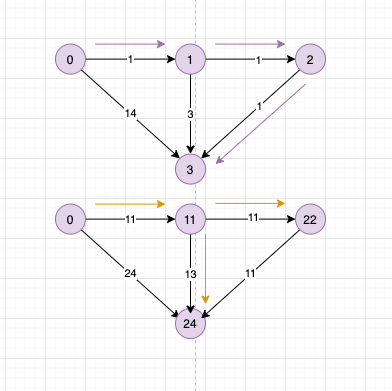
\includegraphics[width=0.5\textwidth]{QQ2.png}
\end{center}

Seen above, by adding 10 to all edges between graph 1 and 2 the minimum spanning tree changes and so the addition doesn't don't preserve the minimum spading tree.
\vfill

\newpage

\item (3 points) Suppose we are given a directed graph $G=(V,E)$ where every edge $e\in E$ has a distinct positive length $\ell_e$, and $s$ is a specified source vertex in $V$.  Assume that every vertex in $V$ is reachable from $s$.

{\bf True or False:} \emph{$G$ has at most one shortest-paths tree.}
If true, give a short explanation.
If false, give a counterexample.

\TT{False}: consider.
 \begin{center}
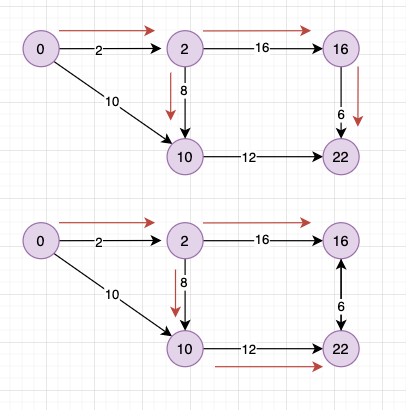
\includegraphics[width=0.5\textwidth]{QQ3.png}
\end{center}

since each path holds the same weight  both are considered a minimum path from s to v making this a valid minimum path tree. 


\vfill

\item (3 points) Suppose we are given a directed graph $G=(V,E)$ where every edge $e\in E$ has a distinct positive length $\ell_e$.
Let $s$ and $t$ be two nodes  in $G$ and let $P$ be a shortest $s \leadsto t$ path in $G$.
Now, suppose we replace the length $\ell_e$ of each edge $e$ by $\ell'_e = \ell_e^2$.

{\bf True or False:} \emph{$P$ is still a shortest $s \leadsto t$ path in $G$ with the new edge lengths.}
If true, give a short explanation.
If false, give a counterexample.

\vfill
\TT{False}

suppose we have the graph.
 \begin{center}
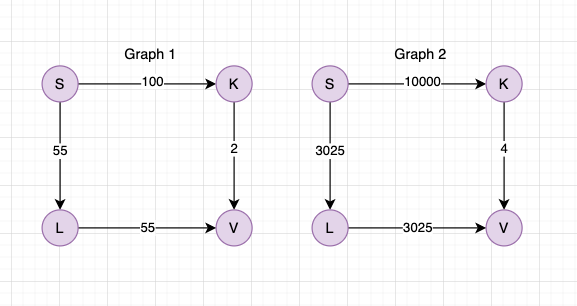
\includegraphics[width=0.5\textwidth]{QQ4.png}
\end{center}
Let P be the shortest path between S and V.
In graph 1 the shortest path from S to V is obviously is $S->K->V = 102$. Now let $\ell'_e = \ell_e^2$.  in graph 2 the shortest path is from S->L->V = 6050 < $100^2 + 2^2$ thus is not the same path after the operation. 



\newpage


\end{enumerate}

\newpage


\problem{Shortest Paths}{15}
Consider the following directed graph, where every edge has a specified length:
\begin{figure}[H]
  \centering
    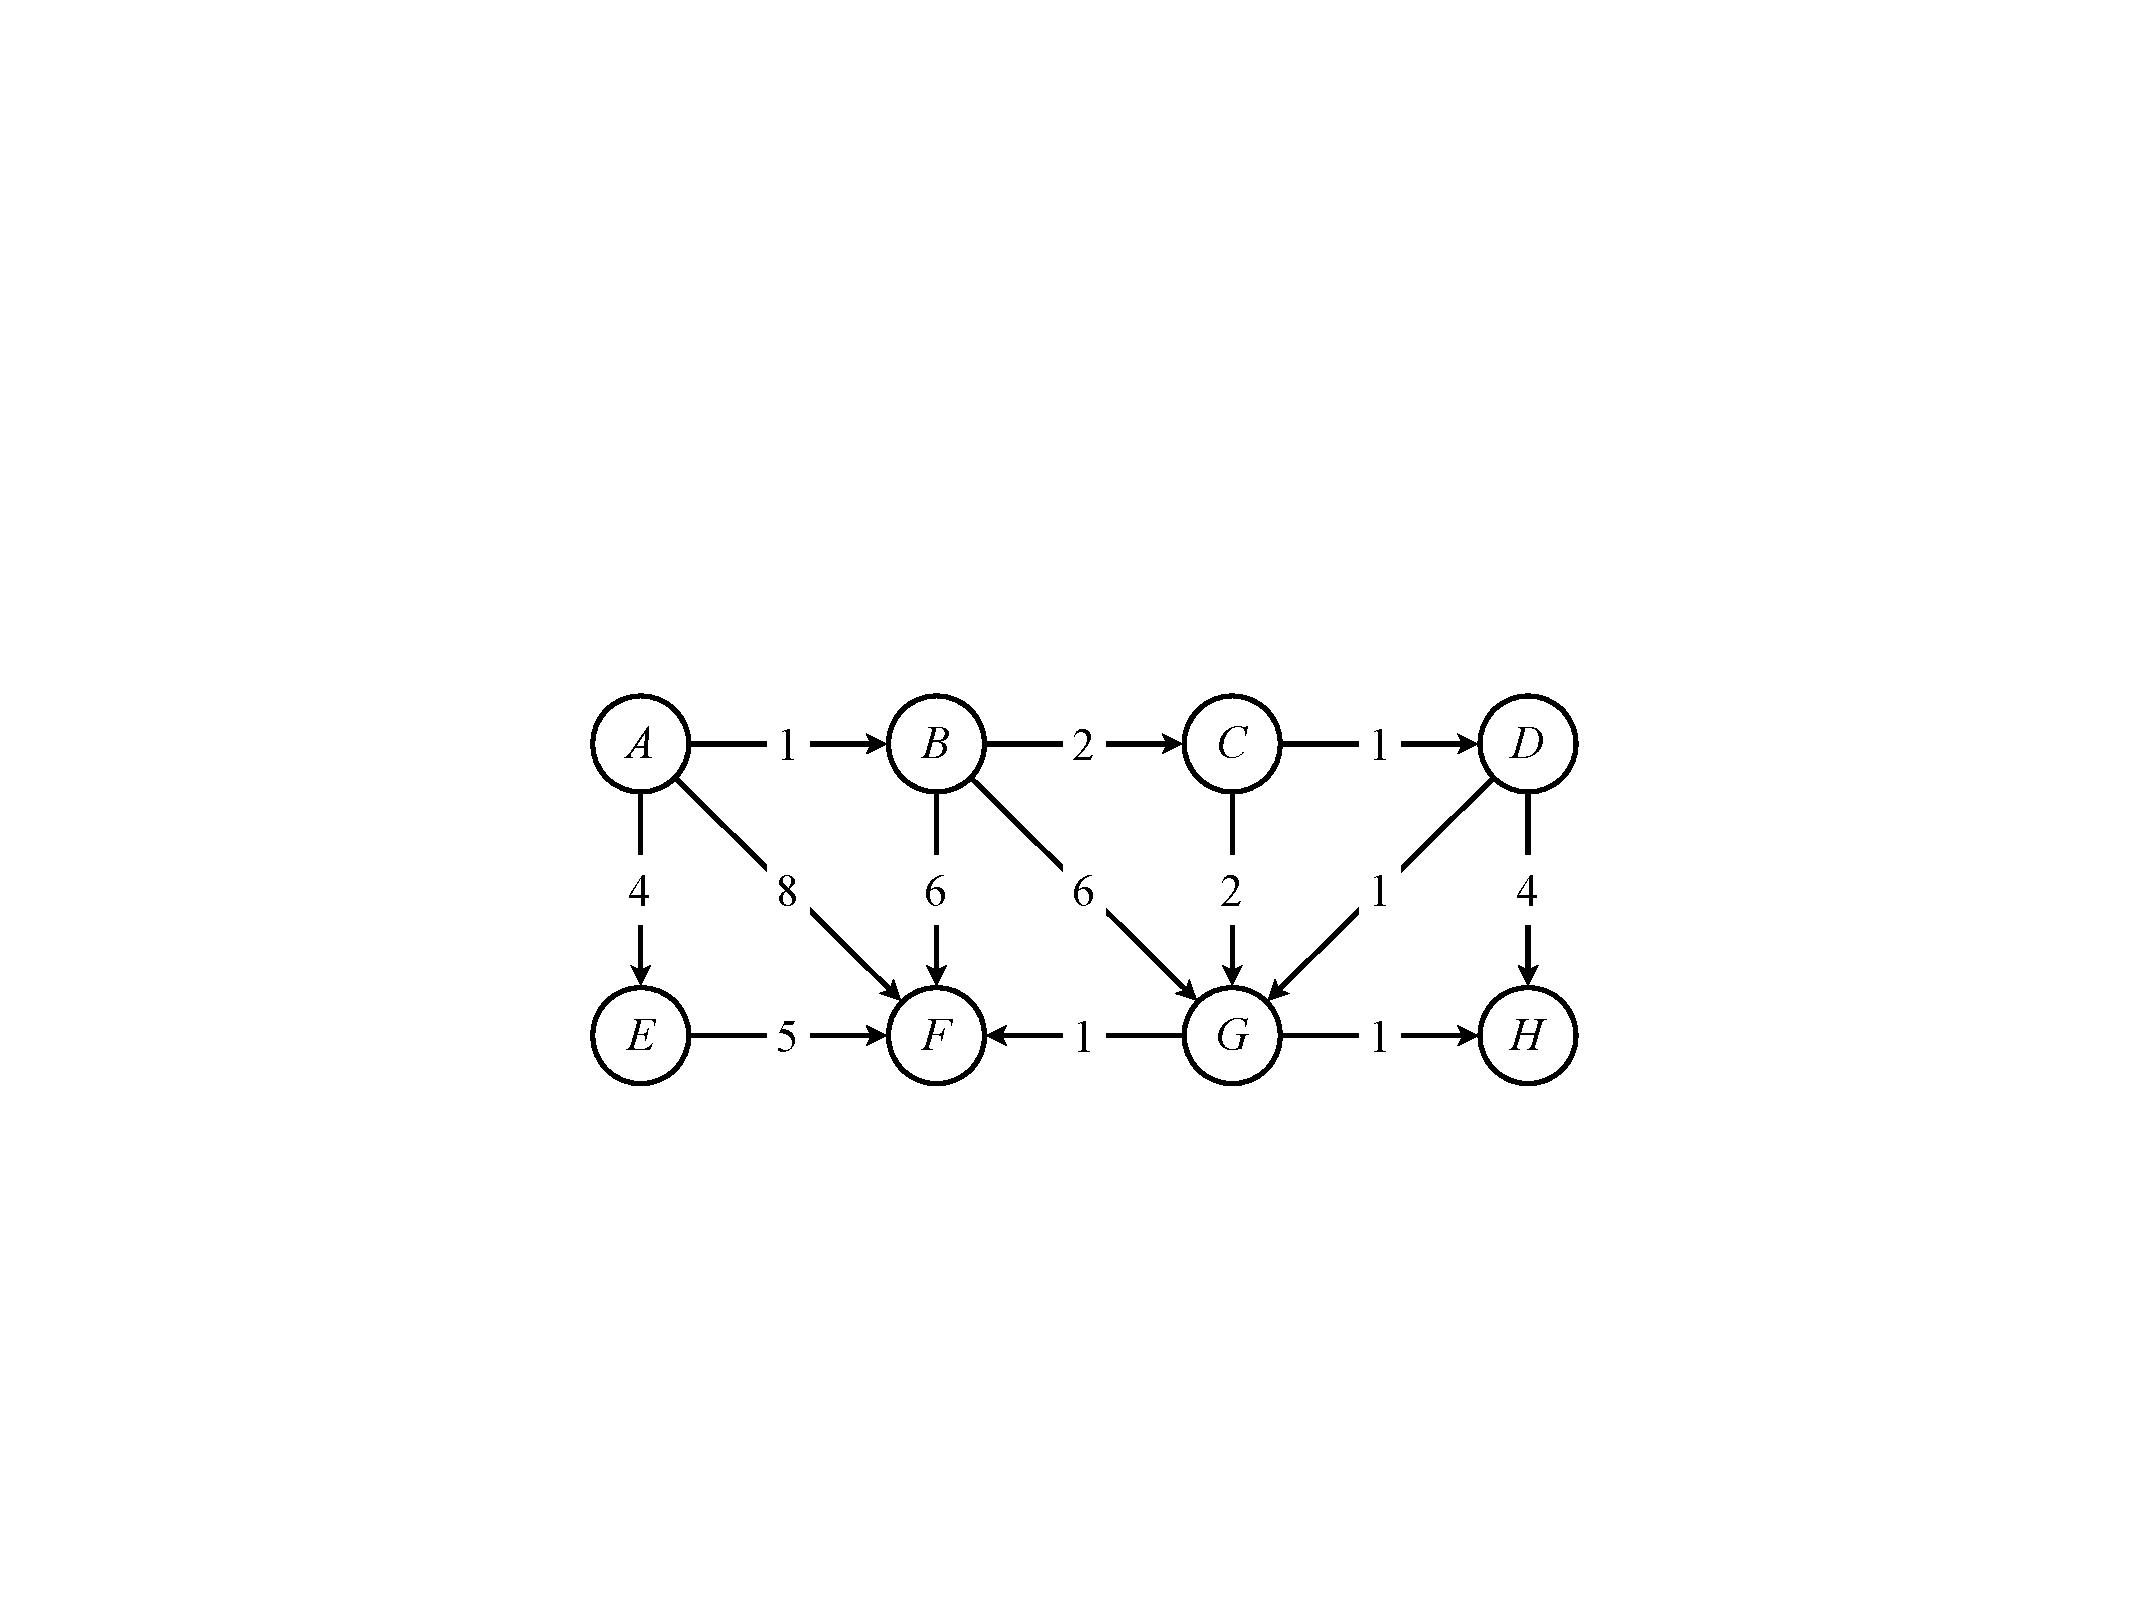
\includegraphics[width=0.4\textwidth]{FIGS/figDijkstra.pdf}
    %\vspace{-20pt}
\end{figure}

\begin{enumerate}[(a)]
\item (10.5 points) Run through Dijkstra's algorithm step-by-step to calculate  shortest paths from $A$ to every other node. 
Show your steps in the following table as the algorithm proceeds.
For example, in the row corresponding to Iteration 1, 
$B$.\texttt{d} 
denotes the 
distance from $A$ to $B$ in iteration 1, and $B$.\texttt{p} denotes the preceding node of node $B$ in iteration 1.
Whenever there is a tie in choosing from a set of nodes, break the tie in alphabetical order.


\begin{table}[h]
\begin{center}
\begin{tabular}{|c||c|c||c|c||c|c||c|c||c|c||c|c||c|c||c|c|} \hline
Iter.\ \# & $A$.\tt{d} & $A$.\tt{p} & $B$.\tt{d} & $B$.\tt{p} & $C$.\tt{d} & $C$.\tt{p} & $D$.\tt{d} & $D$.\tt{p} & $E$.\tt{d} & $E$.\tt{p} & $F$.\tt{d} & $F$.\tt{p} & $G$.\tt{d} & $G$.\tt{p} & $H$.\tt{d} & $H$.\tt{p} \\ \hline \hline
Init.\ & 0 & \tt{Nil} & $\infty$ & \tt{Nil} & $\infty$ & \TT{Nil} & $\infty$ & \TT{Nil} & $\infty$ & \TT{Nil} & $\infty$ & \TT{Nil} & $\infty$ & \TT{Nil}& $\infty$ & \TT{Nil} \\ \hline
1 & 0 & \tt{Nil} & 1 & \TT{A} & $\infty$ & \TT{Nil} & $\infty$ & \TT{Nil} & 4 & \TT{A} & 8 & $A$ & $\infty$ & \TT{Nil} & $\infty$ & \TT{Nil} \\ \hline
2 & 0 & \tt{Nil} & 1 & A & \textbf{3} & \textbf{B} & $\infty$ & \TT{NIL} & 4 & A  & \textbf{7} & \textbf{B} & \textbf{7} & \textbf{B} & $\infty$ & \TT{Nil} \\\hline
3 & 0 & \tt{Nil} & 1 & A & 3 & B & \textbf{4} & \textbf{C} & 4 & A & 7 & B & \textbf{5} & \textbf{C} & $\infty$ & \TT{Nil} \\ \hline
4 & 0 & \tt{Nil} & 1 & A & 3 & B & 4 & C & 4 & A & \textbf{6} & \textbf{G} & 5 & C & \textbf{6} & \textbf{G}\\ \hline
5 & 0 & \tt{Nil} & 1 & A & 3 & B & 4 & C & 4 & A & 6 & G & 5 & C &  6 & G\\ \hline

\end{tabular}
\end{center}
\end{table}%
\begin{proof}[Extra details]
Bold numbers are updated nodes at that level. Now I did not include nodes that did not update any other nodes. For example after 1 we check each B,F,E for other connections and by starting at B we update F in init 2 and then look at F and E. Since F has the lowest path so fare we don't update anything and its left out of the iterations. Below is each node corresponding the its iteration.


1 A\\
2 B\\
E,F nothing happens\\
3 C\\
4 G\\
D nothing happens because H is already updated from G. 
5 H, done\\

shortest path A->B->C->G->H
\end{proof}
\medskip

\item (4.5 points)
Based on the table you filled in for part (a), draw the tree of the shortest paths from $A$ to every other node in the graph.

 The minimal spanning tree of the graph.
 
 \begin{center}
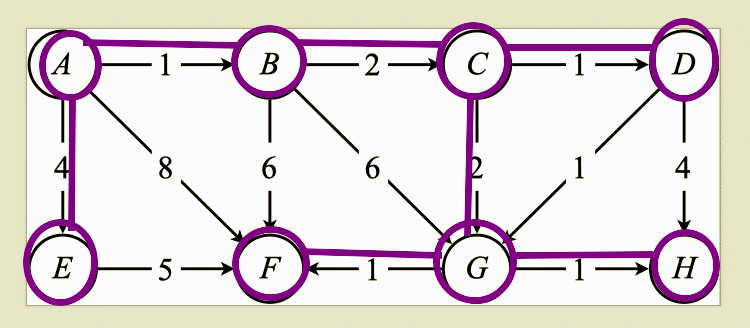
\includegraphics[width=0.5\textwidth]{QQ1.png}
\end{center}


\end{enumerate}


\newpage

\problem{Greedy Algorithms}{15}

Consider a country road that runs in a straight line from East to West  with houses scattered very sparsely along it.   Our goal is as follows.

Solution similar to the interval partitioning this problem can be done by treating cell towers as classes and we want to minimize the number of cell towers.

\begin{quote}
Find a way to place cell phone base stations at certain points along the road, so that every house is within four miles of one of the base stations.  
\end{quote}

\medskip

\begin{enumerate}[(a)]
\item (8 points)

 \begin{algorithm}
\SetAlgoLined
//sort H from least to greatest letting 0 indicate the left most house using Merge.
T = List of Towers 
H = MergeSort(H)\\
int index = 0;\\
\While{|H| > 0}{
$T_{new}$ = new Tower(H[index].position+$4_{miles}$)\\
T.add($T_{new}$ )\\
//remove all nodes in H that are within the bounder of of $T_{new}$\\
h = H[index]\\
	\For{ i = index ; |H| > 0 and h.position <= $T_{new}$.position ; i++}{
		remove h from H\\
		h = H[i]
		index++;
	}
}
return T


 \caption{Greedy Solution(T,H)}
\end{algorithm}

\newpage


\item (4 points)
Justify the correctness of your algorithm (i.e., explain why your algorithm finds the placement that uses the fewest base stations).\\


%----------------------------------------------------------------
Observation: Each tower is a circle of radius 4 miles by at the closes 8 miles from anther tower. This will gives an maximal area covered 

\begin{proof}[Proof of correctness]\;\\


Let T = $\{t_1,...,t_n\}$ be the set of solution created by my algorithm and let Let T' = $\{t_1',...,t_k'\}$ be a set of solutions. let both of else list be sorted from left to right in  starting at index  0 being the left most tower. Now suppose Greedy Solution id not result in the optimal solution. Then there is a $t \in T'$ such that t is not 4 miles from a tower. But we can swap this tower with a tower exactly 4 miles from house t. Over all the T' this can be done to achieve a equivalent solution or better solution. This Greedy Solution creates a optimal solution 
	
\end{proof}
\vfill

%----------------------------------------------------------------

\item (3 points)
Analyze the running time of your algorithm.
\begin{proof}[Solution]
	There are two worst case scenario one is if all nodes are within the first tower, and the second is if all nodes are more then 4 miles apart. 
	
	scenario 1:
		
		Then the running time starts with mergeSort taking O(nlogn). Then the while loop is accessed once. with in the while loop the remove loop removed all nodes running in O(n) since inside the this loop runs in consent time. Thus running in O(nlogn+n) = O(nlogn)
			
	
	scenario 2: 
		Then the running time starts with mergeSort taking O(nlogn). then this while loop runs n times each time deleting one element.  making the run time O(nlogn). As seen there is a compilation between removing elements inside the while loop and the Max number of iterations the while loop and make. 
		
		Thus the worst case is always O(nlogn). 
	
	
	
\end{proof}

\vfill
\end{enumerate}



\newpage



\problem{Unique Shortest Paths}{15}

We are given an undirected graph $G = (V, E)$ where each edge $e \in E$ has a length $\ell_e > 0$, and a starting vertex $s \in V$.  Let $n=\ |V|$ and $m = |E|$. Suppose that, in addition to \dist\ and \pred\ fields, each node $u \in V$ has a Boolean field $u.\usp$.  Give a $O((m + n) \log n)$-time algorithm that, for each node $u \in V$, sets $u.\usp$ to \true\ if there is a unique shortest path from $s$ to $u$; otherwise, it sets $u.\usp$ to \false. (\emph{Note:} $s.\usp == \true$.)

\begin{enumerate}[(a)]
\item (8 points)
Pseudocode of your algorithm:

We can achieve this algorithm by modifying dijkstra's algorithm with a binary heap. 

 \begin{algorithm}
\SetAlgoLined
List<priority queue>  queue\\
\For{each vertex u} {
    u.dist = $\infty$\\
    u.pred = null;
  }   
queue.inset(s)\\
s.distance = 0\\
\While{queue is not empty}{
	u = queue.ExtractMin()\\
	\For{iterate threw all children of u}{
		node child = adjacent vertices\\
		\eIf{child.dist != $\infty$}{
			// check shortest path and usp\\
			\If{child.dist > u.dist + weight}{
				child.dist = u.dist + weight\\
				minheapify(queue)\\
				child.pred = u\\
				child.ups = True\\
			}\ElseIf{child.dist = u.dist + weight}{
				child.ups = False\\
			}	
		}{
			child.dist = u.dist + weight\\
		 	queue.insert(u)\\	
		 	child.pred = u\\
			child.ups = True\\	
		}
	}
	
		
		
}

 \caption{usp(node s)}
\end{algorithm}


\newpage

\item (4 points)
Brief justification for your algorithm:

Threw Dijkstra's algorithm we visited every node and every path within the graph. Then all we need to do is update all nodes usp while visiting nodes if we visit a node with the same path its path is currently not unique and will be set to false. This value will be override if we find a shorter path to x node making x.usp = True. 
 
By setting ups True when first seeing a node we can guarantee later on that if we find a path with the same dist we change ups to false. 
 
\vfill

\item (3 points)
Running time analysis for your algorithm:
%Now each insert, extractMin, and decreaseKey operation takes O(lg n) time, and so the totel time for Dijkstra's algorithm is O((n + m) lg n)\\


By using a priority queues with a binary heap we know that 
Insert, DecreaseKey, ExtractMin , and heapify all run in $O(logV)$). so " V  + V calls to insert + V calls to ExtractMin() + E calls to minheapify" giving us $O(v +(2V+E)logv) = O((2n+m)logn) = O((n+m)logn)$

Minheapify is called when every a child dist is changed inside the queue thus it can only happen with respect the number of Edges inside the graph. 

\vfill

\end{enumerate}

\newpage

\problem{Dynamic Programming}{10 Extra Credit}

\begin{framed}
\begin{center}
\textbf{Note.}  \emph{For this problem, there is \textbf{no} partial credit for answering "I don't know."}
\end{center}
\end{framed}

\medskip

Andy's (a pizza chain) is considering opening a series of restaurants along Scenic Valley Highway (SVH). The $n$ possible locations are along a straight line, and the distances of these locations from the start of SVH are, in miles and in increasing order, $m_1, m_2, \dots , m_n$, where each $m_i$ is a positive integer. The constraints are as follows:
 \begin{itemize}
\item At each location, Andy's may open at most one restaurant. The expected profit from opening a restaurant at location $i$, $i \in \{1,2, \dots , n\}$, is $p_i$, where $p_i > 0$.
\item Any two restaurants should be at least $k$ miles apart, where $k$ is a positive integer.
\end{itemize}

Give an efficient dynamic programming algorithm to compute the maximum expected total profit subject to the given constraints.

\medskip


\begin{enumerate}[(a)]
\item (3 points)
Derive the Bellman equation for this problem:



\vfill

\item (2 points)
Brief justification for your algorithm:


\vfill

\newpage
\item (3 points)
Pseudocode of your algorithm based on the derived Bellman equation in Part (a):

\vfill

\item (2 points)
Running time analysis for your algorithm:

\vfill

\end{enumerate}



\end{document}
